\section{Auswertung}
\label{sec:Auswertung}
In der folgenden Tabelle sind alle Messwerte aufgeführt
Die Temperaturverläufe sind in dem folgenden Diagramm dargestellt und mit einer
linearen Ausgleichstrechnung approximiert.
\subsection{Aufgabe. a}
%\usepackage{pdfpages}
%  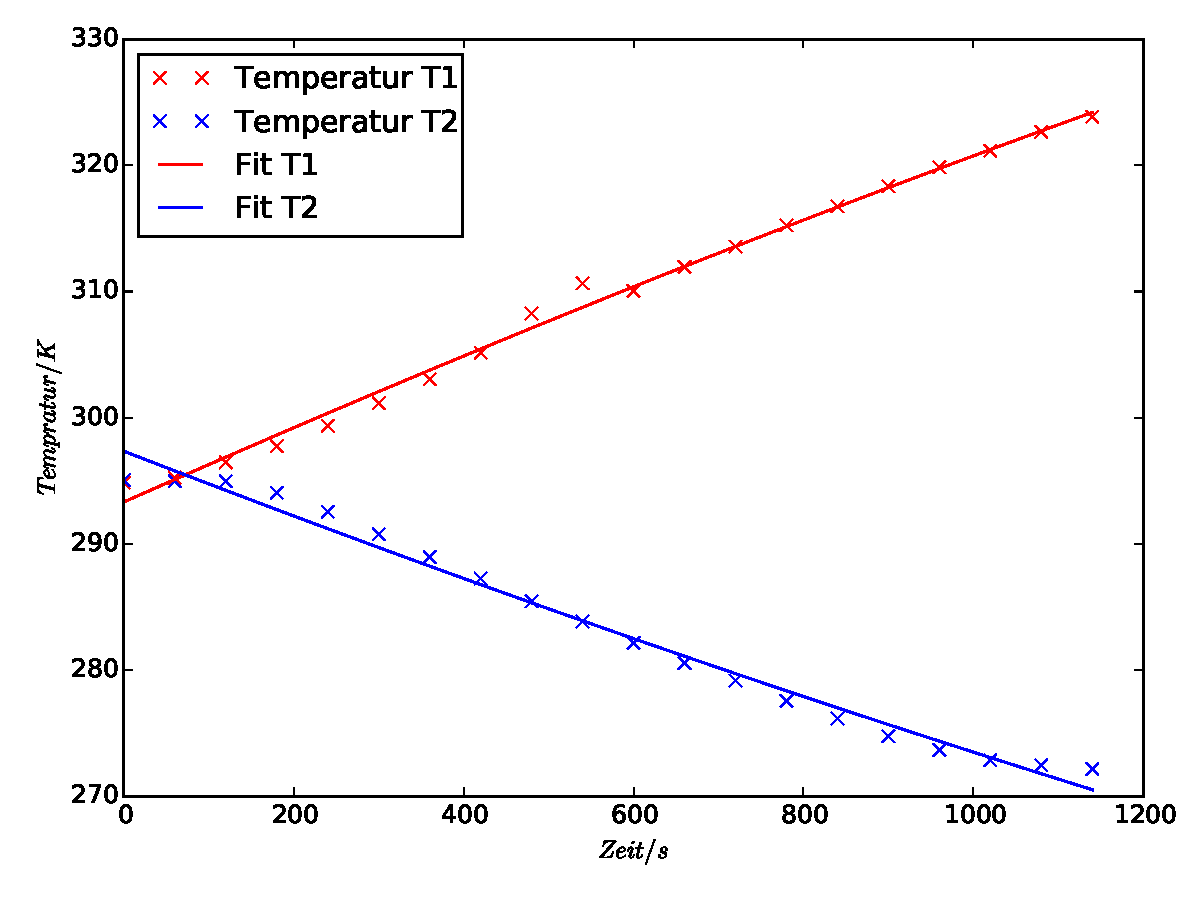
\includepdf[pages=-]{Temperaturgraphik.pdf}
Die Näherung wurde mit scientific Python gemacht und ist gegeben durch
\begin{equation}
  T(t)=At^2+Bt+C .
\end{equation}
Die Parameter für erwärmte Reservoir $T_1$ sind
\begin{equation}
  A=(  -0.000002485)\frac{K}{s^2}
  B=(   0.029925168)\frac{K}{s}
  C=( 293.312793014)K
\end{equation}
Die Parameter für den anderen Behälter$T_2$ sind
\begin{equation}
  A=(  0.000002259)\frac{K}{s^2}
  B=( -0.026112097)\frac{K}{s}
  C=(297.339350549)K

\end{equation}
\begin{table}
  \centering
  \caption{Messdatentabelle.}
  \label{tab:Data}
  \begin{tabular}{c c c c c c}
    \toprule
    $t/s$ & $T_1/K$ & $T_2/$ & $p_a/\text{bar}$ & $p_b/\text{bar}$ & $N/W$\\
    \midrule
    0  &  21.7  &  21.9  &  4.1  &   4.2  &  170 \\
    1  &  22.1  &  21.8  &  1.4  &   6.0  &  170 \\
    2  &  23.3  &  21.8  &  1.8  &   6.2  &  180 \\
    3  &  24.6  &  20.9  &  2.0  &   6.7  &  190 \\
    4  &  26.2  &  19.4  &  2.1  &   7.2  &  195 \\
    5  &  28.0  &  17.6  &  2.1  &   7.3  &  200 \\
    6  &  29.9  &  15.8  &  2.1  &   8.0  &  200 \\
    7  &  32.0  &  14.1  &  2.1  &   9.0  &  205 \\
    8  &  35.1  &  12.3  &  2.1  &   9.5  &  205 \\
    9  &  37.5  &  10.7  &  2.1  &   9.9  &  208 \\
   10  &  36.9  &   9.0  &  2.1  &   9.4  &  210 \\
   11  &  38.8  &   7.4  &  2.1  &  10.7  &  208 \\
   12  &  40.4  &   6.0  &  2.1  &  10.0  &  208 \\
   13  &  42.1  &   4.4  &  2.1  &  10.4  &  210 \\
   14  &  43.6  &   3.0  &  2.1  &  10.9  &  210 \\
   15  &  45.2  &   1.6  &  2.2  &  11.0  &  210 \\
   16  &  46.7  &   0.5  &  2.2  &  11.5  &  210 \\
   17  &  48.0  &  -0.3  &  2.2  &  12.0  &  210 \\
   18  &  49.5  &  -0.7  &  2.2  &  12.1  &  210 \\
   19  &  50.7  &  -1.0  &  2.2  &  12.5  &  210 \\
   \bottomrule
 \end{tabular}
\end{tabel}
